\subsection{Tabla comparativa}
Debido a la gran cantidad de navegadores, nuestra página debe ser accesible pero además debe mostrarse bien dentro de la amplia gama de navegadores actuales:\\
\begin{table}[htbp]
	\begin{center}
		\begin{tabular}{|l|l|}
			\hline
			Navegador & Diferencia \\
			\hline \hline
			Chrome & Reproductor de audio con apariencia distina. \\ & Necesario instalar Flash player para animación \\ \hline
			Firefox & Reproductor de audio con apariencia distina. \\ & También necesita Flash player \\ \hline
			Explorer & Reproductor de audio con apariencia distina. \\ & También necesita Flash player \\ \\ \hline
			Safari & Reproductor de audio con otra apariencia.  \\ & Algunos errores de estilo \\ &(Version 2012) \\ \hline
			Konkeror & Problemas con archivos multimedia. \\
			& (Audio, Flash Player) \\ \hline
		\end{tabular}
		\caption{Comparaciones.}
		\label{tabla:sencilla}
	\end{center}
\end{table}\\

\subsubsection{Google Chrome}
\begin{figure}[h]
	\centering
	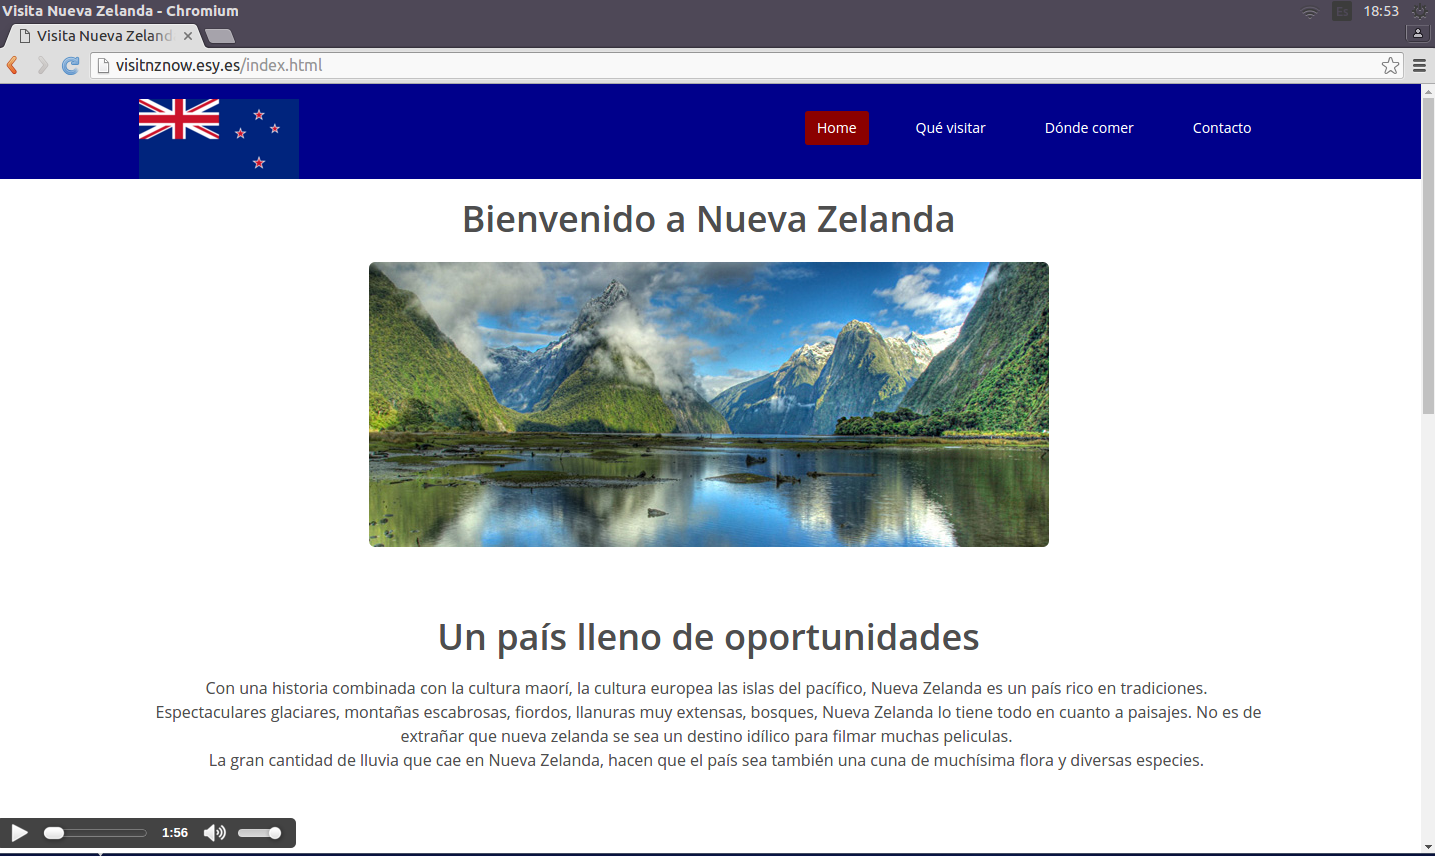
\includegraphics[width=0.95\textwidth]{./Fotos/chrome-capture.png}
	\caption{Captura de la página principal en Chrome}
	\label{fig: ejemplo}
\end{figure}
Como podemos observar, el aspecto es muy similar. El navegador necesitará tener instalado Adobe Flash Player para que se muestre la animación realizada en "animoto". \\ \\ También hay diferencias en el reproductor por defecto del navegador para el audio de nuestra página principal.
\subsubsection{Mozilla firefox}
\begin{figure}[h]
	\centering
	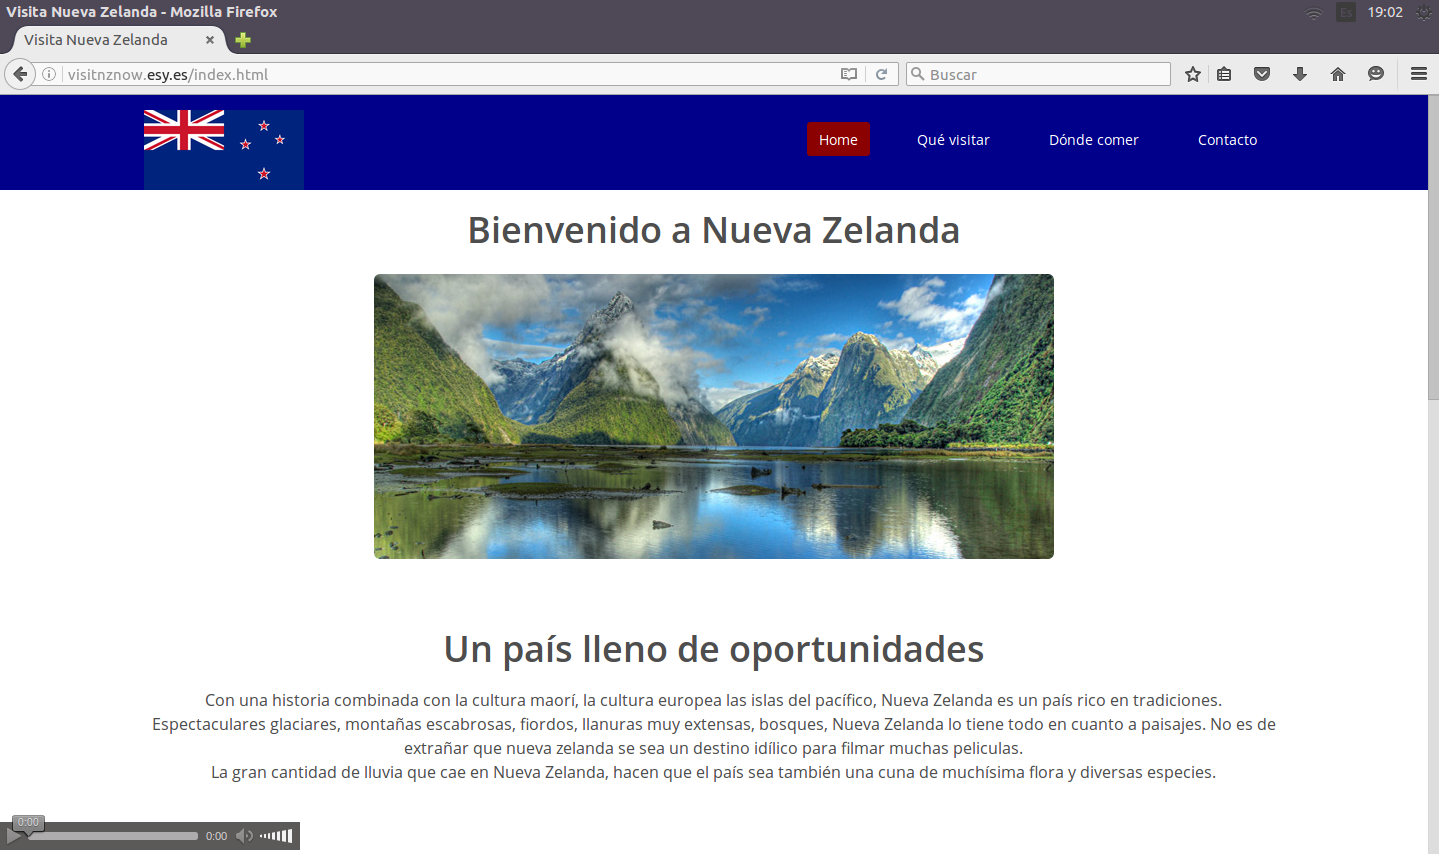
\includegraphics[width=0.95\textwidth]{./Fotos/firefox-capture.png}
	\caption{Captura de la página principal en firefox}
	\label{fig: ejemplo}
\end{figure}
Al igual que en chrome, es necesario instalar Adobe Flash player si no está instalado, para mostrar la animación. La apariencia del reproductor de audio cambia con respecto a Chrome.
\subsubsection{Internet explorer}
\begin{figure}[h]
	\centering
	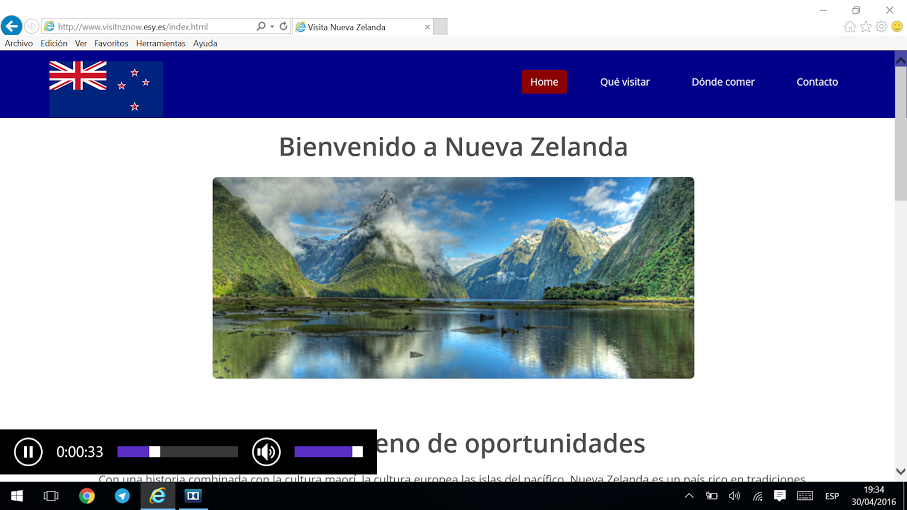
\includegraphics[width=0.95\textwidth]{./Fotos/explorer-capture.png}
	\caption{Captura de la página principal en explorer}
	\label{fig: ejemplo}
\end{figure}
En internet explorer también cambia el reproductor de audio. Con nuestro diseño hemos conseguido que también sea 100\% funcional en este navegado
\subsubsection{Opera}
\begin{figure}[h]
	\centering
	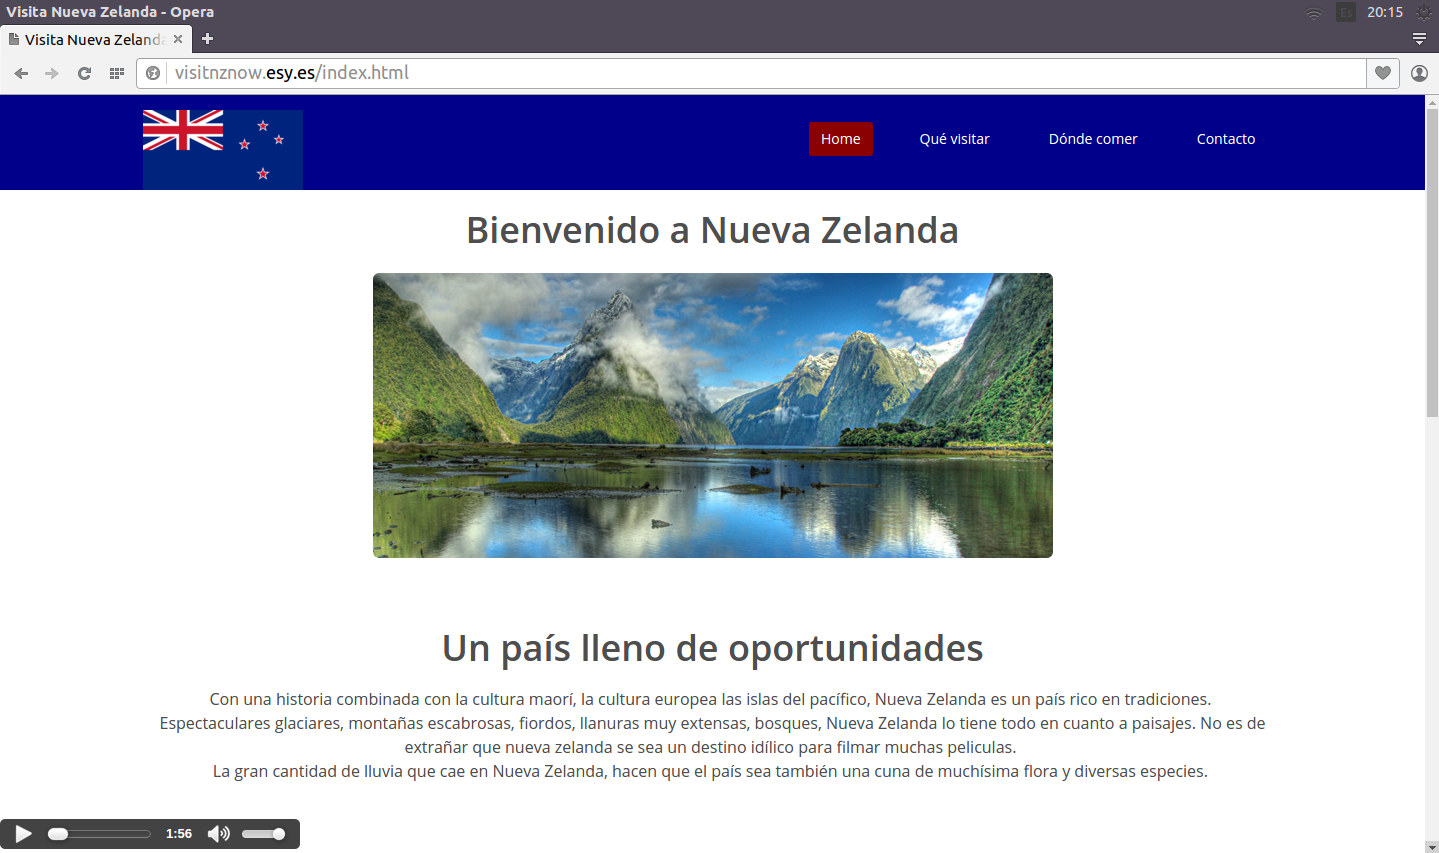
\includegraphics[width=0.95\textwidth]{./Fotos/opera-capture.png}
	\caption{Captura de la página principal en opera}
	\label{fig: ejemplo}
\end{figure}
Con respecto a los otros navegadores no se ha encontrado ninguna diferencia, salvo el reproductor que es identico al de Chrome.
\subsubsection{Safari}
\begin{figure}[h]
	\centering
	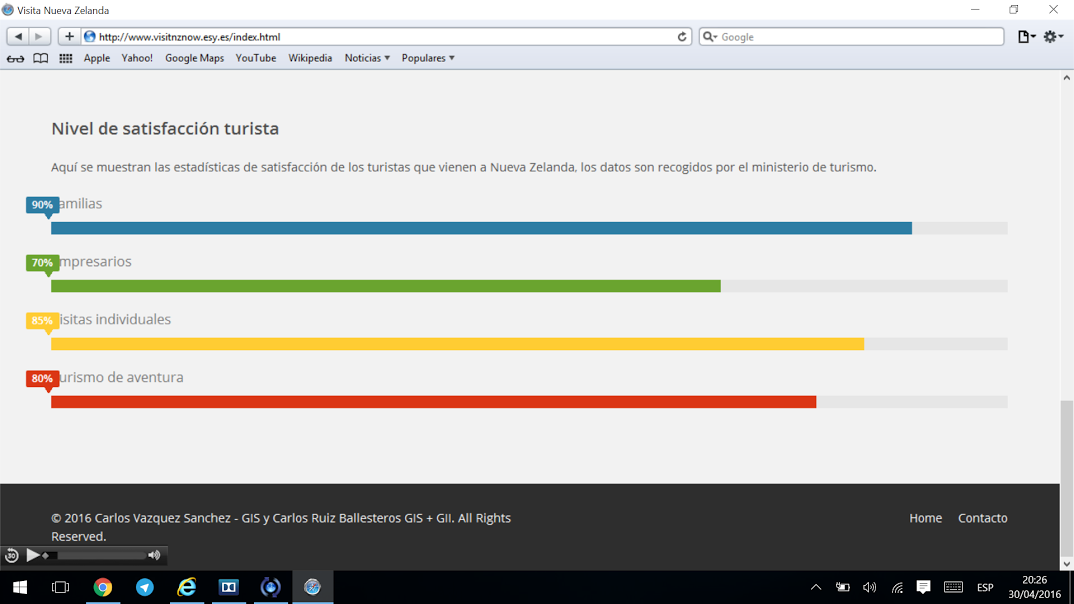
\includegraphics[width=0.95\textwidth]{./Fotos/safari-capture.png}
	\caption{Captura de error de estilo en Safari 1 - 2012}
	\label{fig: ejemplo}
\end{figure}
\begin{figure}[h]
	\centering
	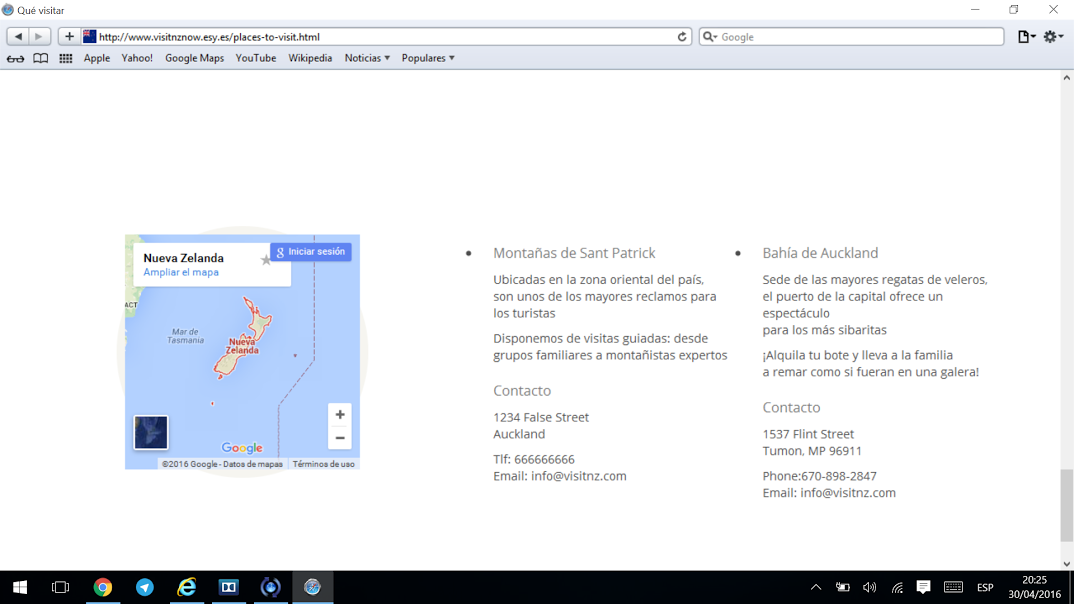
\includegraphics[width=0.95\textwidth]{./Fotos/safari2-capture.png}
	\caption{Captura de error de estilo en Safari 2 - 2012}
	\label{fig: ejemplo}
\end{figure}
En safari hemos tenido que utilizar la última versión que hizo Apple para windows, ya que no disponemos ninguno de los integrantes del grupo de un Mac. Se pueden apreciar 2 errores de estilo. El primero, que el porcentaje no aparece al final de la barra de progreso, y el segundo lo podemos ver en la sección de Google Maps que hemos puesto en el sitio web, que no aparece en forma de circulo. 
\subsubsection{Konqueror}
\begin{figure}[h]
	\centering
	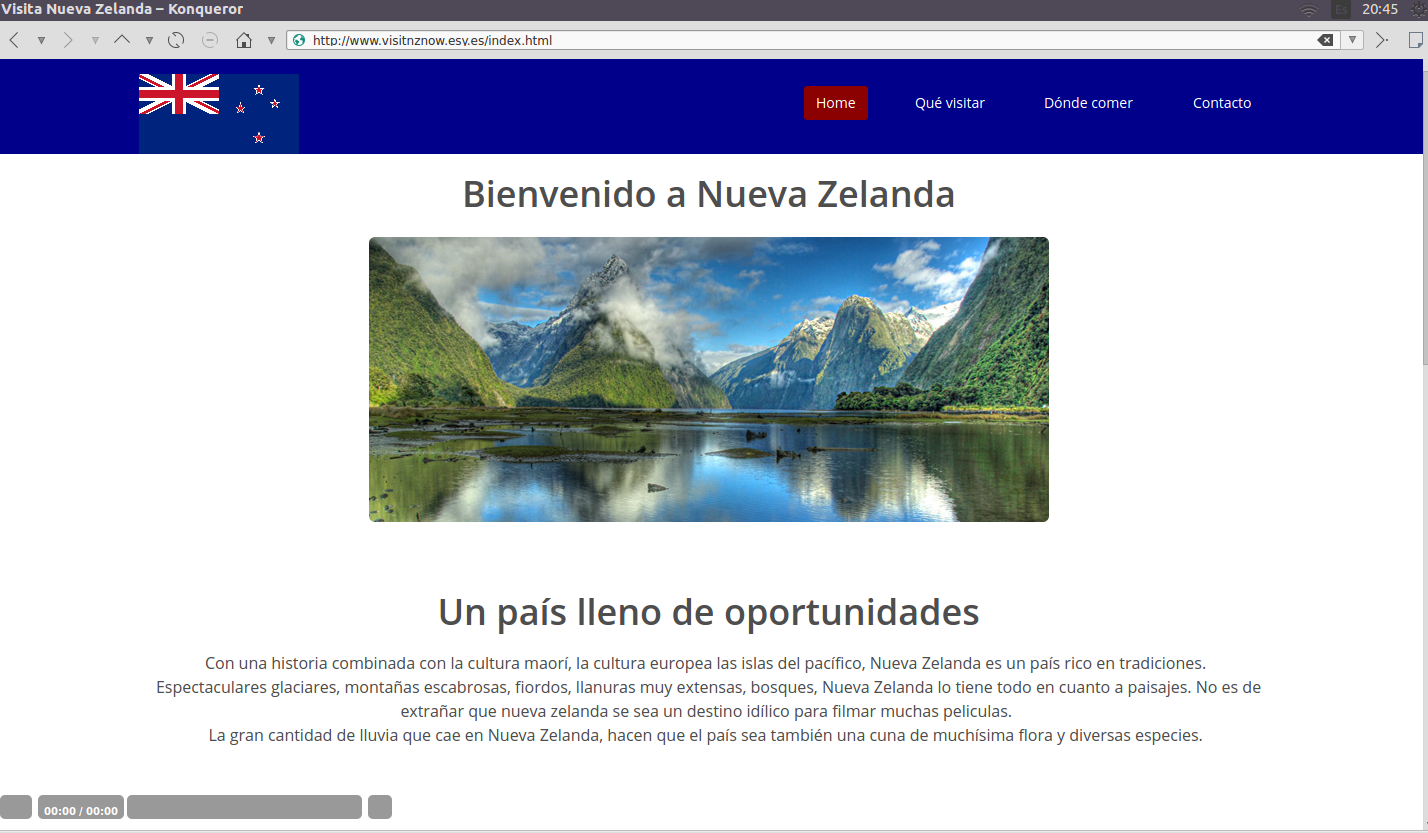
\includegraphics[width=0.95\textwidth]{./Fotos/konqueror-capture.png}
	\caption{Captura de la página principal en Konqueror}
	\label{fig: ejemplo}
\end{figure}
Konqueror ha sido incapaz de leer el audio y la animación en Flash Player. Aún así el reproductor de audio sale, pero sin ningún recurso cargado.
\subsection{Descripción de las principales dificultades}
La mayoría de las dificultades que hemos encontrado ha sido la de cumplir con los estándares de accesibilidad del W3C. Por un lado algunas de las herramientas de verificación(En concreto TAW), no nos identificaba el tag ``audio'' y lo señalaba como error cuando es un tag de html5. \\ \\
Por otro lado el hecho de tener distintas herramientas para comprobar la accesibilidad nos ha ayudado bastante en dejarlo lo más adecuado posible. \\ \\
Además el diseño responsive con los "iframe" también daba algunos problemas hasta que hemos encontrado los estilos adecuados para que se pueda ver en cualquier resolución y en cualquier dispositivo sin ningún problema.
\\ \\Y para finalizar, tenemos que mencionar las pruebas con safari. No disponíamos de ningún ordenador Mac, por lo que tuvimos que utilizar la última versión que realizó Apple sobre Windows para probar la página.
\subsection{Análisis personal y conclusiones}
Tras realizar esta práctica nos hemos percatado de todos los puntos que hay que tener en cuenta a la hora de desarrollar una página con un buen nivel de accesibilidad. Aspectos como la navegación textual, el contraste o tamaño del texto, los efectos sonoros y visuales que a priori a nosotros no nos presentan ningún impedimento pueden convertirse en una barrera infranqueable para un determinado perfil de usuario.\\
Por ello todos estos puntos nos han hecho reflexionar sobre las diferentes capacidades que pueden tener los usuarios de nuestro software, así de la necesidad de tenerlos siempre en cuenta a la hora de desarrollar software.